\documentclass[tikz]{standalone}
\usepackage{amsmath}
\usetikzlibrary{positioning,3d,calc}

\begin{document}

\begin{tikzpicture}

\node (obs) at (0, 0) {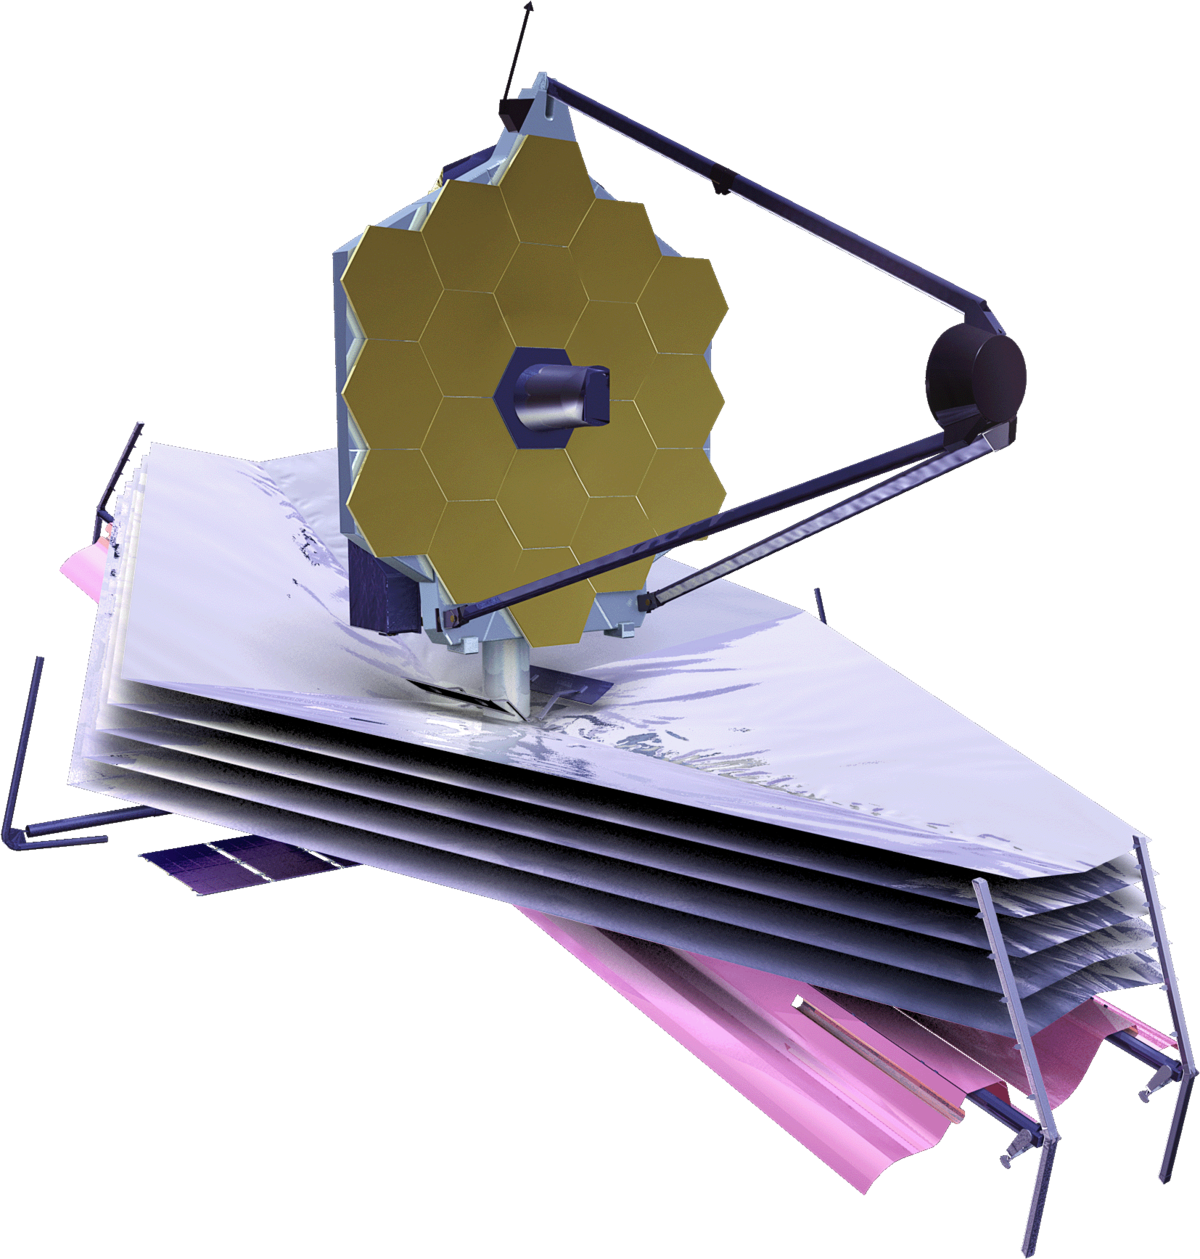
\includegraphics[width=1cm]{jwst_spacecraft}};

\draw (2, -0.5, -1) -- ++(0, 1, 0) -- ++(0, 0, 1) -- ++(0, -1, 0) -- ++(0, 0, -1); 
\draw (4, -0.5, -1) -- ++(0, 1, 0) -- ++(0, 0, 1) -- ++(0, -1, 0) -- ++(0, 0, -1); 

\draw[latex-latex] (0, -1.2) -- (4, -1.2) node[midway, below] {$D_{s}$};
        
\end{tikzpicture}
\end{document}
